\lipsum[1-1]

\begin{figure}[h!]
	\centering
	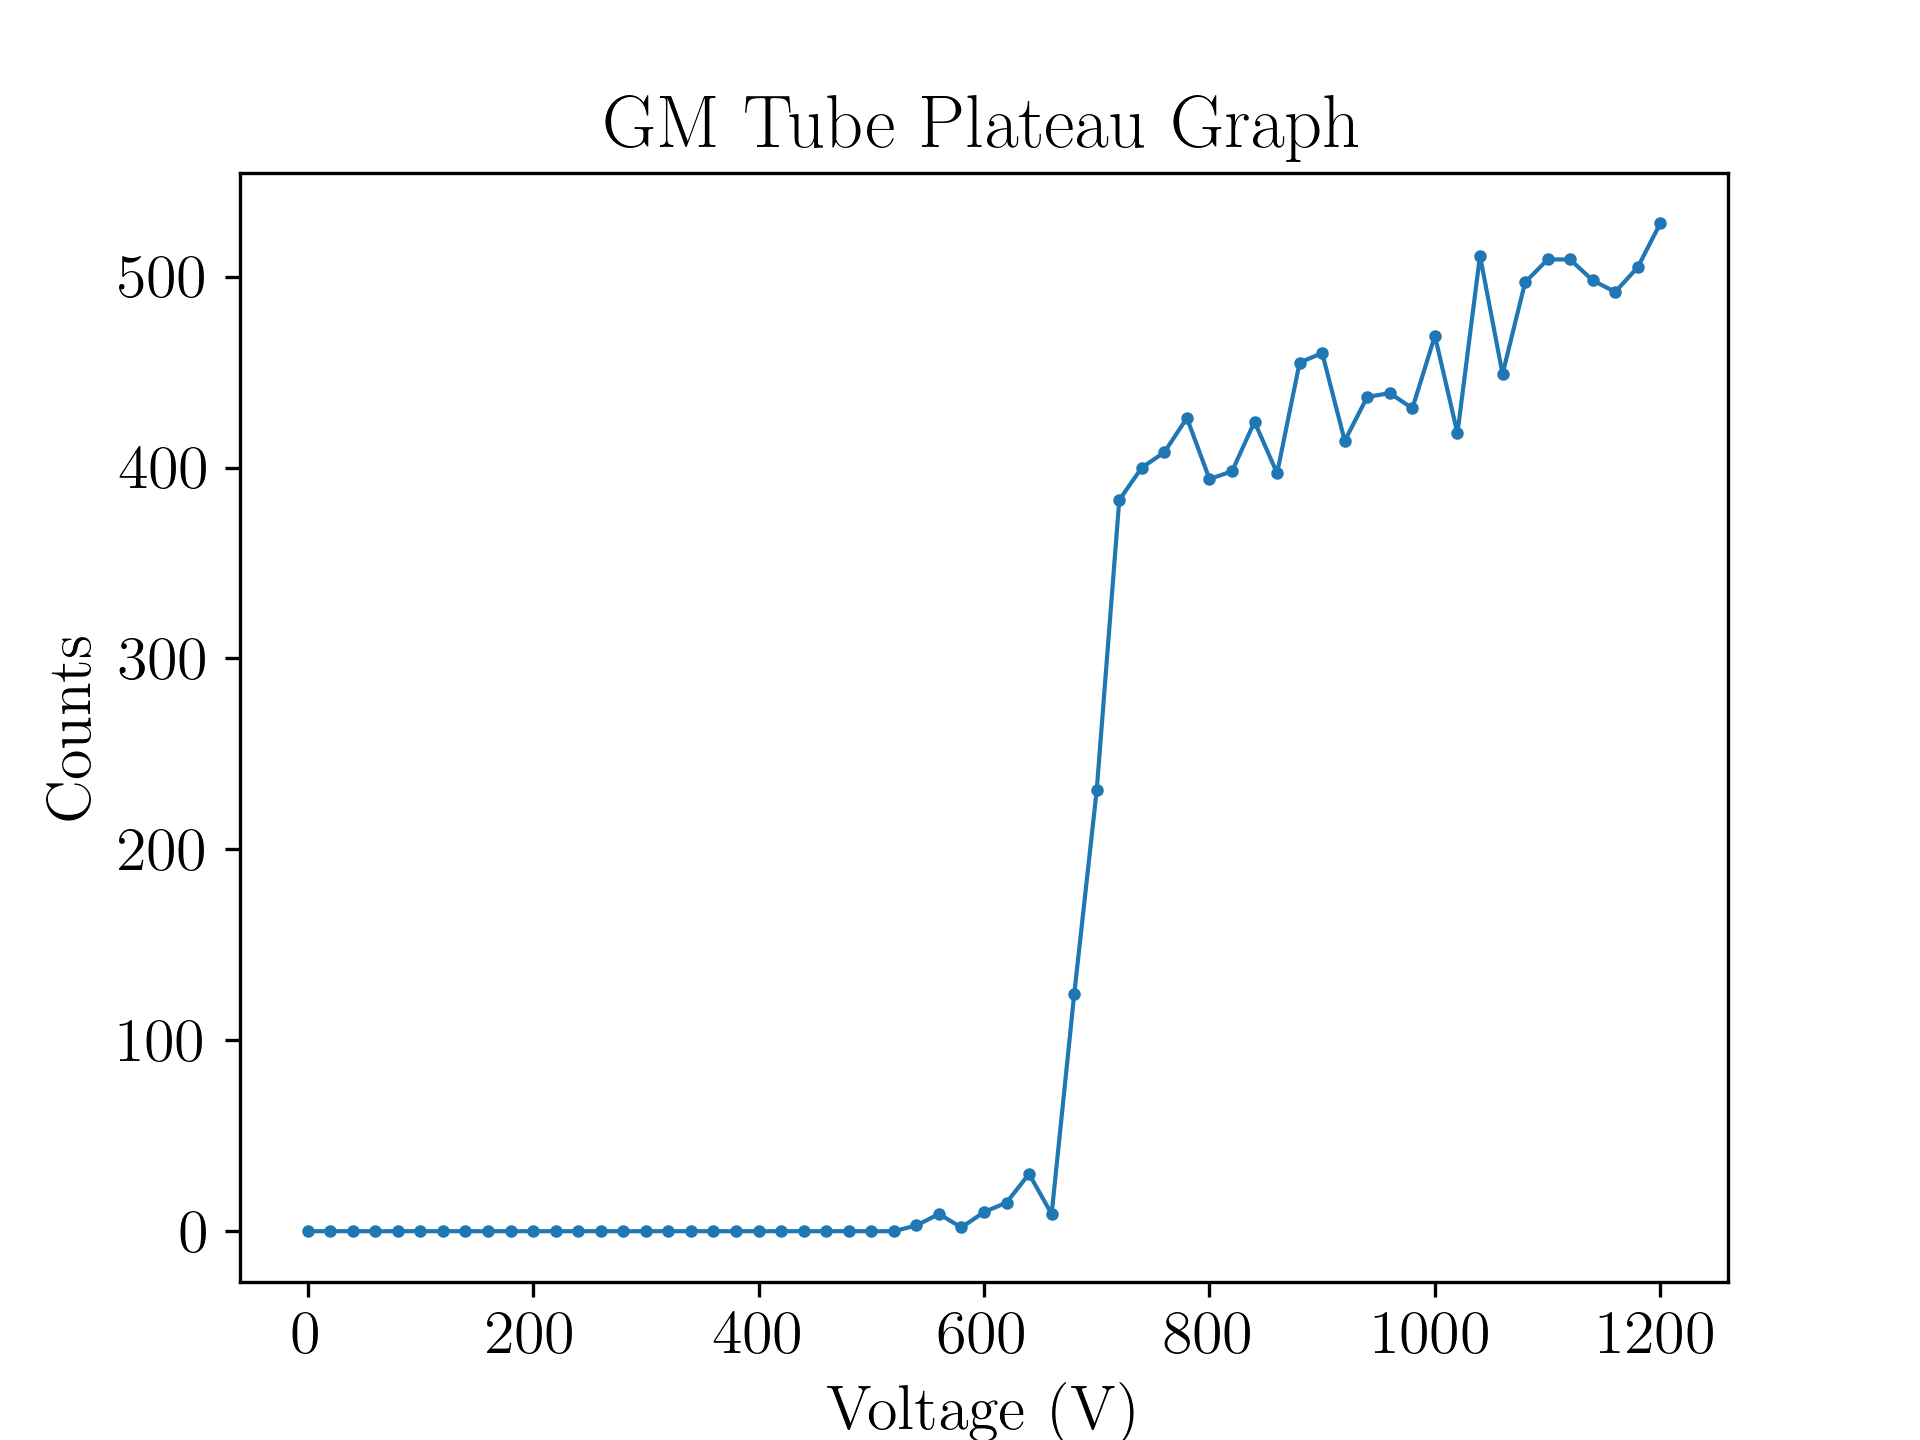
\includegraphics[scale=1]{PlateauGraph.png}
	\caption{Counts vs. Voltage (V) for the plateau curve experiment, where the operating voltage of the Geiger-Muller tube was increased by 20 V from 0 V to 1200 V.}
\end{figure}

\begin{figure}[h!]
	\centering
	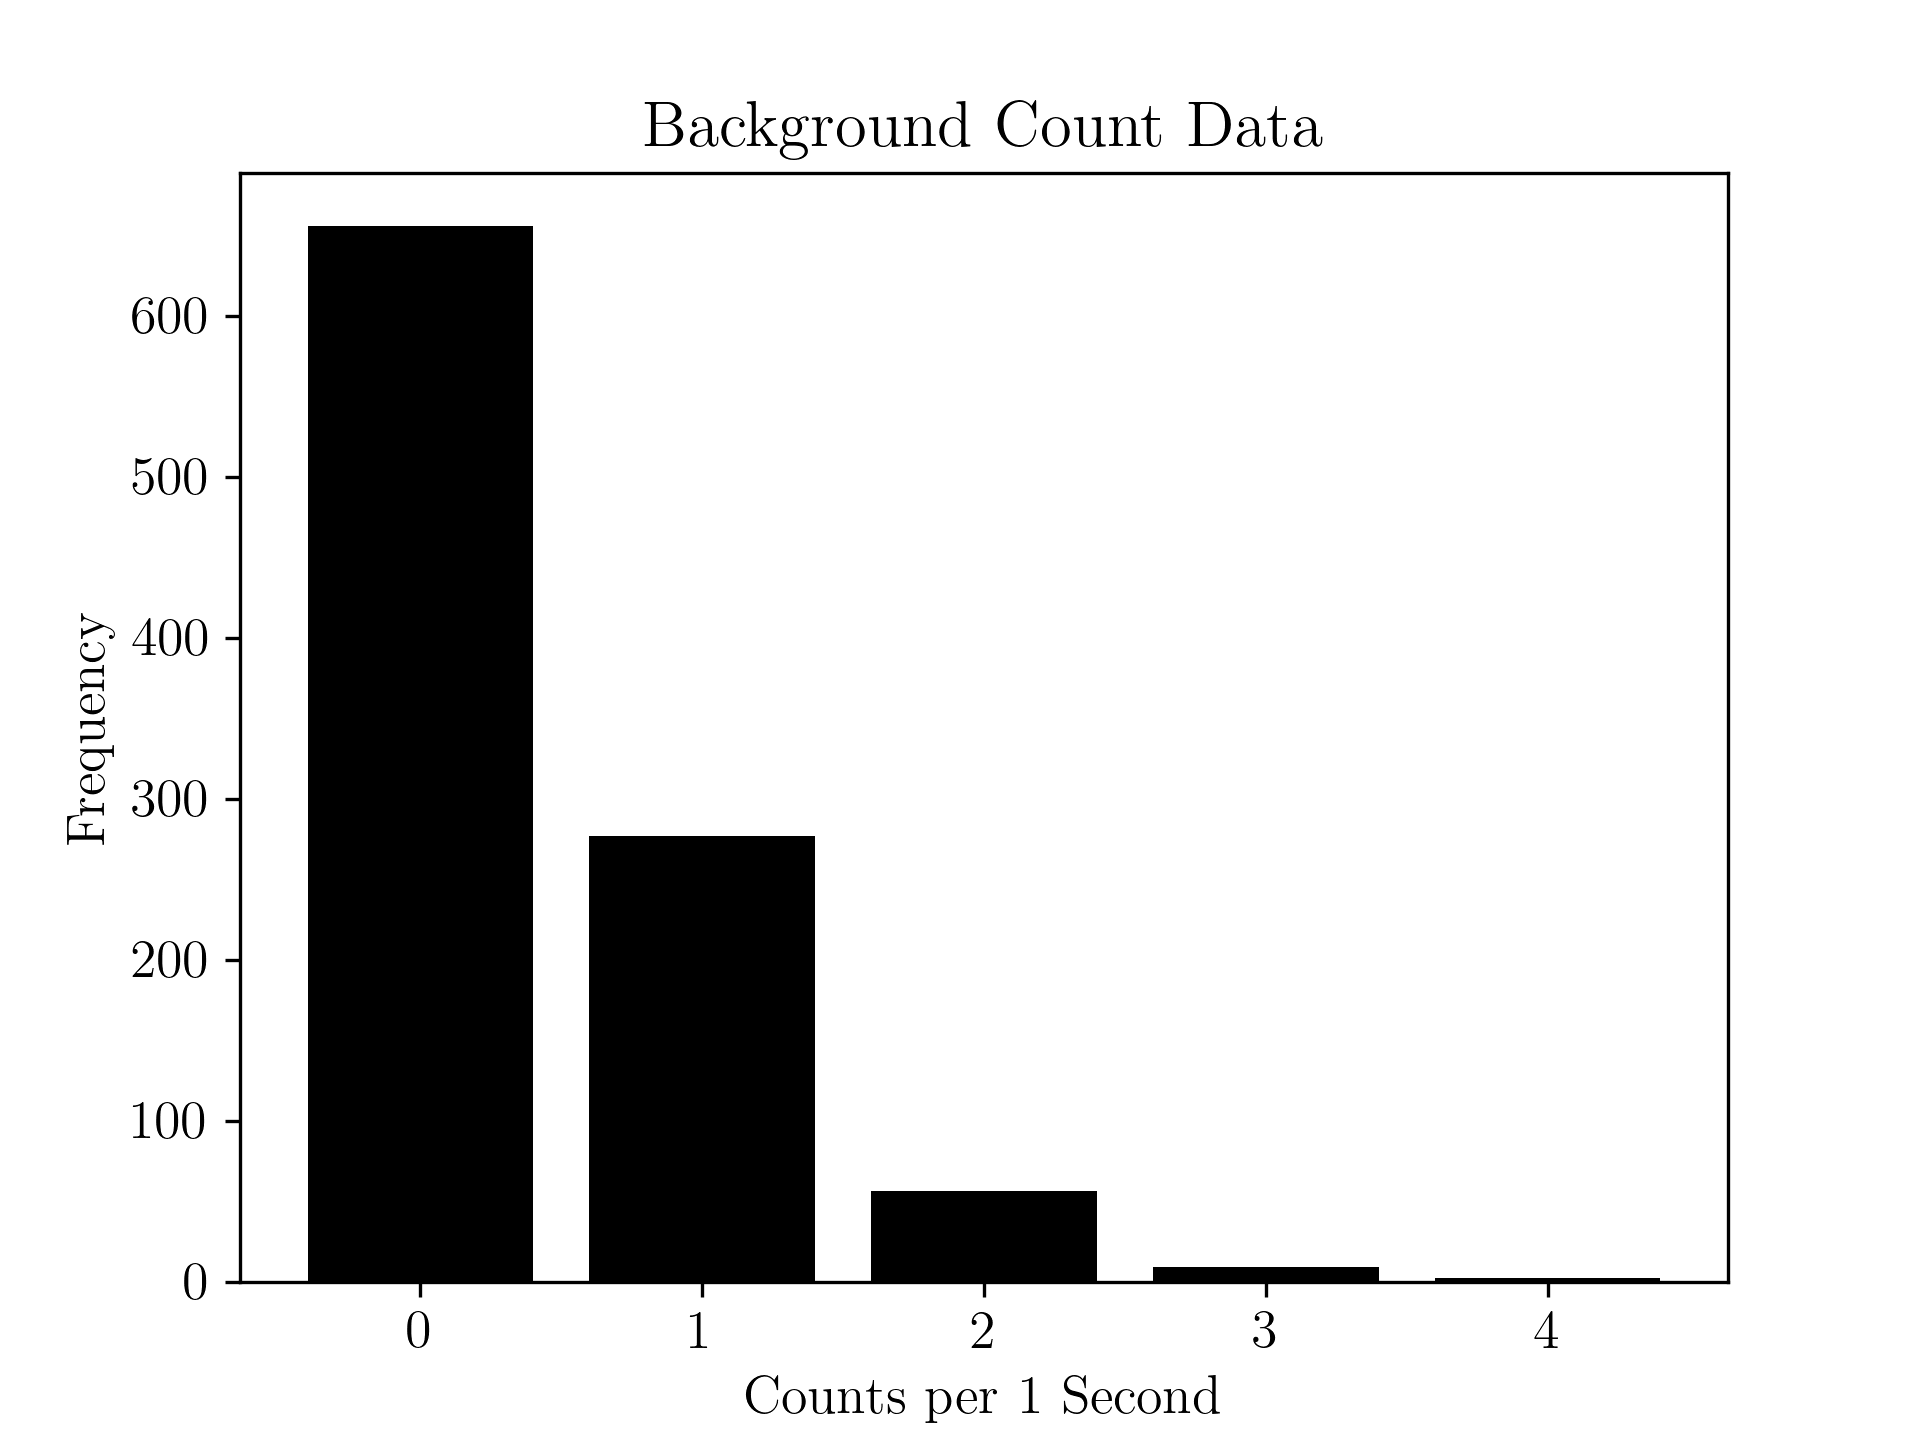
\includegraphics[scale=1]{BackgroundCountHist1sec.png}
	\caption{Count distributions over intervals of 1 second for the background measurement.}
\end{figure}

\begin{figure}[h!]
	\centering
	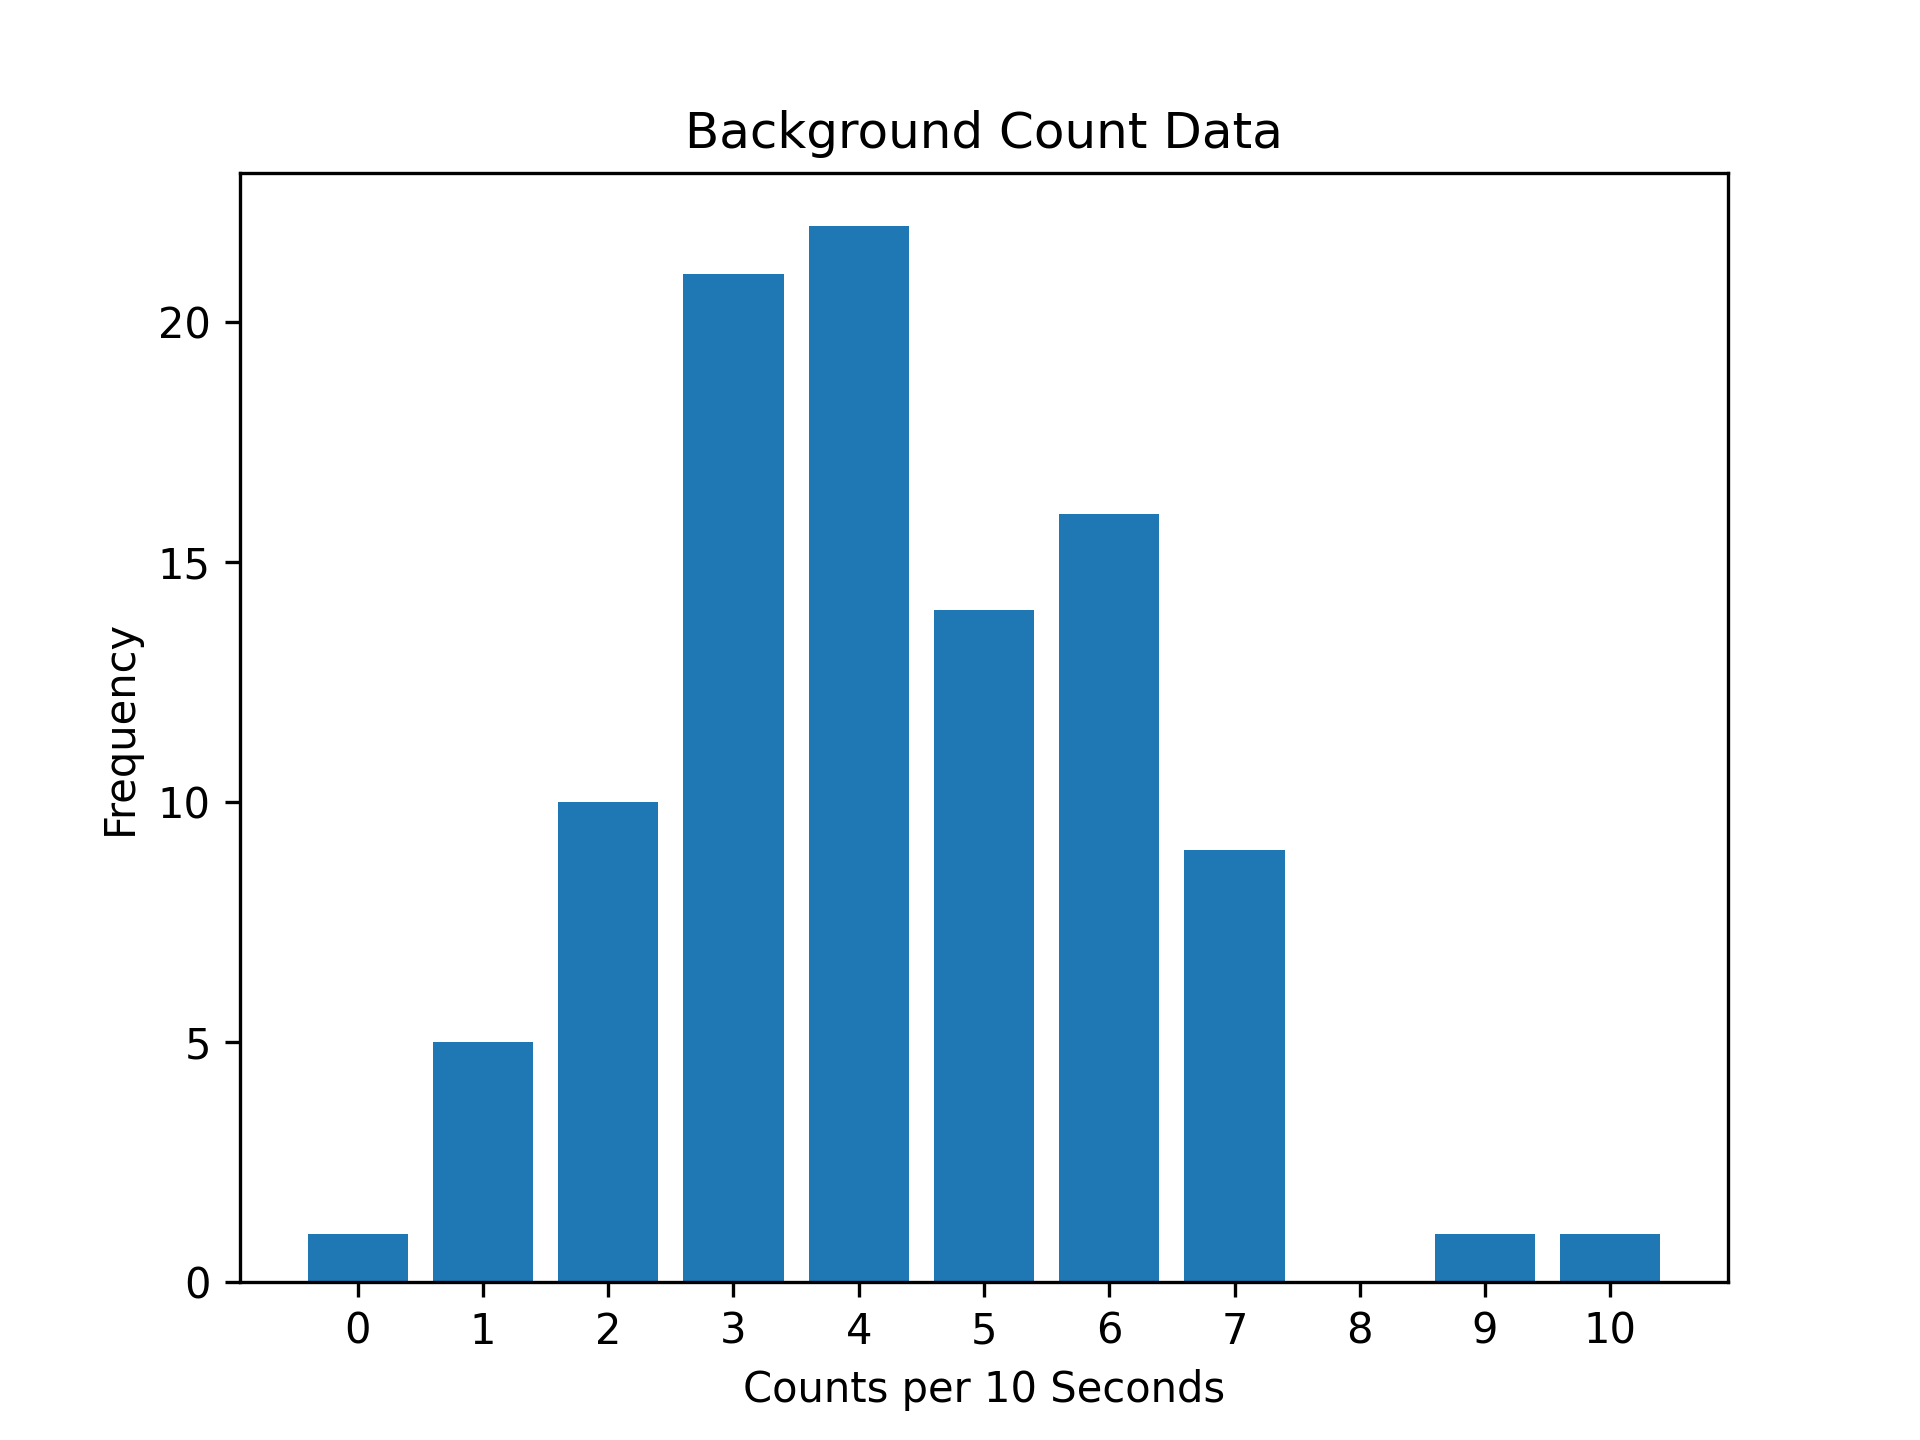
\includegraphics[scale=1]{BackgroundCountHist10sec.png}
	\caption{Count distributions over intervals of 10 seconds for the background measurement.}
\end{figure}

\begin{figure}[h!]
	\centering
	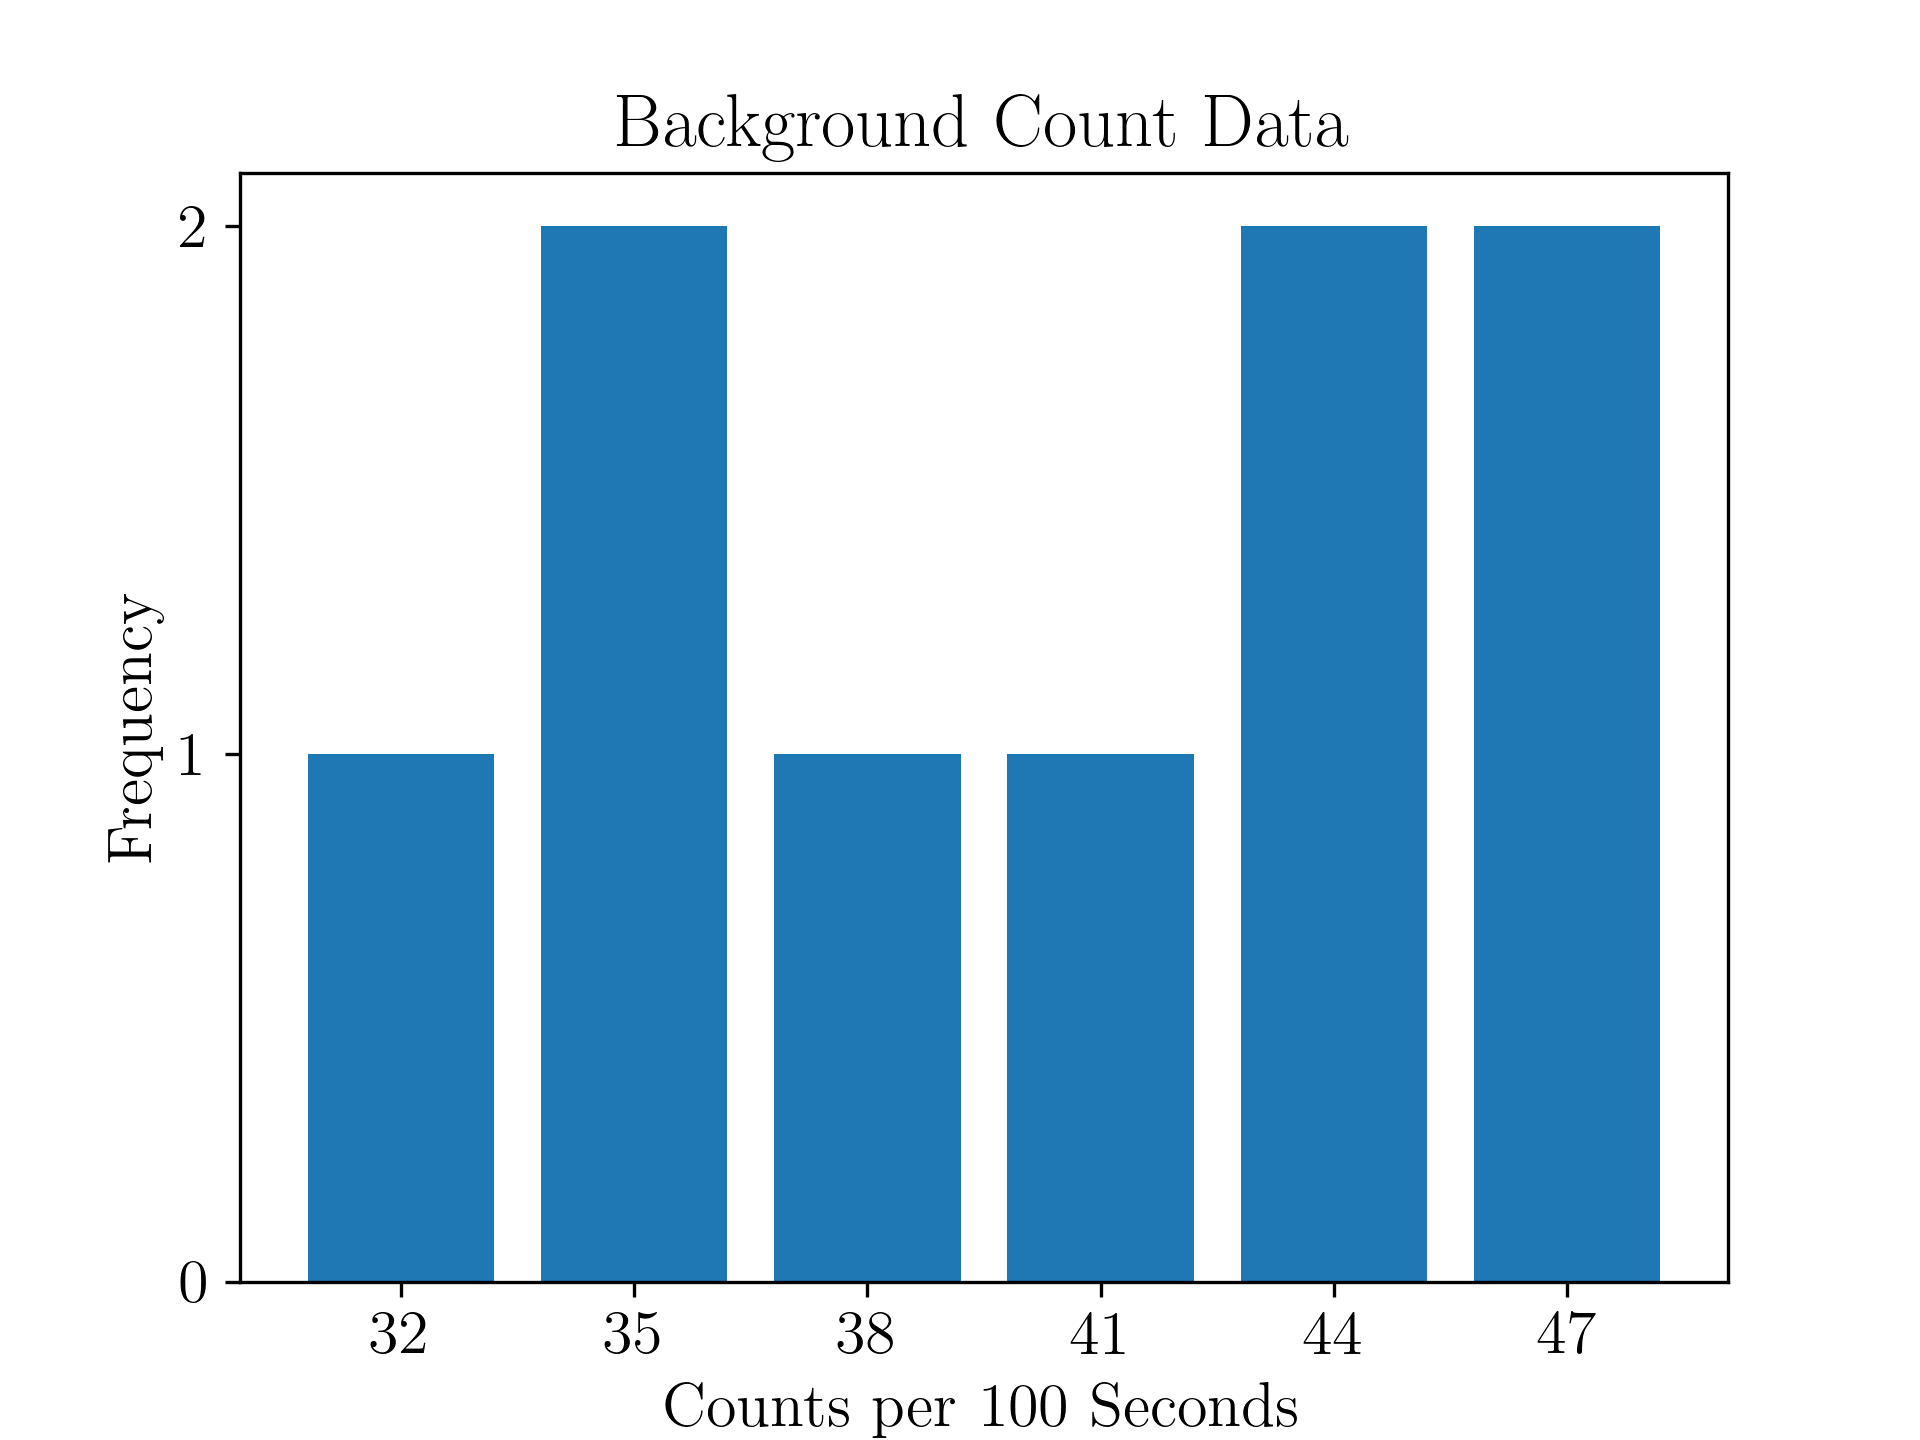
\includegraphics[scale=1]{BackgroundCountHist100sec.png}
	\caption{Count distributions over intervals of 100 seconds for the background measurement.}
\end{figure}


